\chapter{Simulation Optimisation with Aspect Orientation}\label{chap:exp1_simulation_optimisation}

With a game deployed to experiment participants and a dataset of empirical play
collected, it was possible to determine optimal play in any game state. This
entirely separate body of work is documented in another student's PhD
thesis\inline{Cite William's PhD thesis}. This dataset leads to
further research. If we understand how players \emph{should} play, and we have
data to indicate how they \emph{do} play, we can investigate how real-world
players might be modelled. 

\section{Aims}\label{sec:aop_simulation_optimisation_aims}

Aspect orientation's use in previous simulation and modelling efforts have
typically focused on the use of aspects to compose model or simulation
details\inline{There must be tons of good citations for aspects being used to
compose together a simulation / model}\revnote{We don't think this is the case
--- those citations just don't exist! Rework to discuss use of AOP in business
process modelling, and note that nobody made those models in practice, just tooling.}.
Critics of aspect orientation note that
the act of process composition makes visually understanding codebases difficult,
and so ensuring that a simulation properly models real-world behaviour is made
trickier with the introduction of aspect orientation. However, aspect
orientation might instead be used to \emph{augment} an existing model, by
rethinking what aspects are used to represent.

An alternative use of aspects would be to first build a non-aspect-oriented
model of \emph{expected} behaviour, and separately build aspects which describe
deviations from this. For example, one might more realistically simulate safety
procedures by first producing an idealised, ``naive'' model of what employees
are expected to do, and separately model alterations to prescribed behaviour as
an employee's boredom, expectation that checks and balances are unneccesary
wastes of their time, and so on --- effectively, separating out models of
degraded modes\cite{johnson2007degradedmodes}.

Previous research on the use of aspect orientation to model degraded modes
adopted the traditionally claimed benefit of aspect orientation: separation of
cross-cutting concerns, allowing for a greater reusability of
codebases\cite{wallis2018caise}. A repository of cross-cutting concerns in
socio-technical simulation such as boredom was developed as a library to be
applied to any future models\cite{fuzzimoss_repo}. However, aspects used in
simulation have no intrinsic need to represent concerns that are cross-cutting.
Indeed, whether they can be accurately used to represent cross-cutting concerns
in simulation is the topic addressed in \inline{Add a cross-reference to the
chapter on cross-cutting concern simulation accuracy when it exists}. Aspects
might instead be used to represent \emph{amendments to processes} which deviate
from an expected norm, in this case represented by the idealised model aspects
are applied to.

To more concretely relate this to the experiment at hand: play of RPGLite can be
modelled as players matchmaking, picking characters, and then mutually taking
turns until one player's characters are entirely expired. Once a player's
characters are dead, new matches can be made. This can continue indefinitely.
Lacking a heuristic to select next moves or characters, players might be
modelled as picking random moves. However, heuristics for move selection can be
added to the naive model of play by way of augmenting the processes already
defined through aspects. This approach can be of significant utility in both
modelling player behaviour and accurately modelling different players:

\begin{enumerate}
    \item Different players might use their own unique heuristics to model play.
    Each player's behaviour is therefore well described by separating what play
    ``looks like'' to what makes a given player play differently to their peers.
    \item Different players might lean more heavily on different heuristics, or
    mixes thereof. Play might be characterised by reliance on experience, on
    recent games, on knowledge of an opponent, and so on; these different
    variables can be expected to be weighted differently by each player, adding
    complexity to the code which models this individualised play.
    \item A modeller might discover a new idea for a heuristic long after
    developing an original concept for a model. Due
    to the impact of \pointno{2}, ideal architectures for an approach such as
    this should allow these heuristics to be defined entirely separately to
    the base model to maximise flexibility when maintaining experiments.
\end{enumerate}

Considering \pointno{1}, \pointno{2}, and \pointno{3}, architectures and
paradigms which enable separation of concerns are well-suited to defining
alternative approaches to play. Some architectural approaches such as mixins or
plugin design patterns might support this structure well, but they typically
rely on language features (in the case of mixins) or knowledge of software
engineering (in the case of design patterns). Aspect orientation is typically
provided to developers as a framework or runtime in a language (such as
AspectJ\cite{aspectj_intro} or PROSE\cite{popovici2002PROSE}) and can require
minimal architectural understanding to use: concepts are simple, and the effort
of composition is alleviated by the supporting framework or runtime.

The approach makes little use of aspect orientation's significant contribution
--- cross-cutting concerns --- as whether behaviour cross-cuts different parts
of a codebase is not of interest in this use case. Instead, aspect orientation
is treated as a composition mechanism with a reasonably low degree of technical
knowledge required.

\subsection{PyDySoFu Suitability}\label{subsec:optimisation_with_aspects_usingpdsf}
Some aspect orientation frameworks do not adequately achieve this requirement.
For example, the most influential framework, AspectJ, requires the use of
language extensions to define integrate aspect
orientation\cite{AspectJLanguageAndTools}, and similar additional complexity is
added in seemingly every alternative framework, through the use of bespoke
virtual machines, compilers, translators, or
languages\cite{rajan2006nu_towardsAO_invocation,popovici2003JITaspects,AspectCplusplusDesignImpl,baker2002maya}.

PyDySoFu, however, requires very little additional knowledge to use. Its design
prioritises simplicity and a shallow learning curve that makes its adoption by
researchers without a software engineering background feasible: \inline{maybe
cut this list of reasons PyDySoFu is fantastic...}

\begin{itemize}
    \item PyDySoFu is implemented as a pure-python library, meaning that it can
    be installed through Python's package manager (pip) and imported like any
    other Python library. No additional supporting infrastructure is required.
    \item Aspects in PyDySoFu are simple functions which take as arguments
    whichever pieces of information are pertinent for the function's use as an
    aspect\footnote{For example, an ``encore'' aspect which is woven after a
    target procedure returns will be provided that target's return value.}.
    \item To weave a PyDySoFu aspect requires only a method call, which returns a
    \lstinline{callable} which unweaves that aspect.
    \item Defining PyDySoFu pointcuts requires only a regular expression
    matching a method name. This can apply to a wide range of join points if
    required, but where method names are provided directly, the join point is
    made clear.
    \item Additional clarity over where aspects \emph{can} be woven is
    introduced by PyDySoFu's transparent weaving of aspect hooks, mitigating
    some of aspect orientation's most prominent criticisms.
\end{itemize}

PyDySoFu therefore satisfies the requirements of this work well: it offers
composition of procedures outside of the scope of an original codebase, makes
what is being composed where clear to a programmer, and makes no significant
changes to Python as a language (thereby requiring users to specialise in fewer
tools). 


\subsection{Proposed Experiment}\label{subsec:optimisation_with_aspects_experiment}

Aspect orientation's use as a composition tool for model components makes sense
in principle, but it is unclear whether the addition of behaviours to a naive
model would make the model more ``realistic''. Furthermore, changes to a model
could alter its representation so as to weaken its mimicry of the system it
simulates; adding behaviours could make it \emph{less} realistic. The
fundamental issue at play is that it is unclear whether the changes made would
properly represent what might be empirically observed. While PyDySoFu's design
makes understanding what is being composed simpler than other aspect orientation
frameworks, a composed model under this paradigm is still split across multiple
areas of a codebase, making a visual assessment of whether a model accurately
reflects the intended behaviour impractical. It is therefore important to
demonstrate the efficacy of PyDySoFu and the modelling paradigm it introduces,
by confirming the realism of a model to which behavioural variation is applied.

We can confirm whether aspects can realistically represent changes to a naive
understanding of the real world by comparing their output against empirical
data. For example, if a such a model of behaviour in a system outputs data which
correlates poorly against empirically collected data, a change to that system
would make it more realistic if it improved this correlation, and could be said
to be realistic if the generated data appeared sufficiently ``close'' to the
empirical dataset --- which here means that the correlation between the two is
of statistical significance. Such a change can be aspect-oriented. Therefore, we
can see the application of aspects as the application of packages of potential
improvements to a base model, which can be verified by way of comparison to
known-good datasets.

This is the basis of the experiments in this thesis.

With datasets collected empirically on RPGLite's play, we can build a naive
model of play and aspects to apply that should realistically model data from
players. This can be used to answer the question:

\begin{researchquestion}
    Can aspect-oriented models be said to exhibit realism?
\end{researchquestion}

% To answer this question, a naive model of play is produced, and aspects
% developed which encapsulate different play styles so as to compare empirically
% sourced datasets against both its aspect-augmented and unaltered counterparts.
% The following subsections detail the naive model developed and aspects applied
% to this model.

To answer this question, a naive model of play is produced. Aspects are
developed which model learning within the system defined by the naive system.
The synthetic datasets produced by models with naive or aspect-applied models
can be compared to an empirical dataset sourced from real-world players of the
game, and their similarity compared. 

``Naive'' is used here to describe a model which does not encode any
understanding of the players of the game being modelled. Traits such as
learning, distraction, or aptitude for similar games are irrelevant to the naive
model. We need a naive model to demonstrate the effectiveness of an
aspect-oriented alternative: we can measure how closely it reflects empirical
data, and compare this against the same measurement drawn from another model
with behavioural variations encoded using aspects. A closer match from our
aspect-oriented model would demonstrate that the technique can enhance a model's
realism. Our naive model also provides a null hypothesis: if no improved
similarity is observed, the technique brought no improvement to the model's
realism. No measurable difference indicates that weaving behavioural variations
as aspects has no impact on a model's realism.

\inline{Write a little here on the learning aspects.}

\inline{Flesh this out as a brief wrap-up of our experimental technique. The end
of our ``naive'' model explanation might be useful to move down here / rework
into this para.} Contrasting the similarity of the empirical dataset to both
naive and aspect-applied datasets\ldots{} This discussion is provided so as to
provide context for the following sections; experimental design is discussed in
more depth in \cref{sec:optimisation_with_aspects_experimental_design}. 


\section{Naive Model}\label{sec:optimisation_with_aspects_naivemodel}

A naive model of play was developed by separating each stage of the actions
taken by players in the client-side app, and separating them into individual
procedures. 

To facilitate the retrieval of information pertinent to a simulation in an
applied aspect, the model was written so as to contain simulation state as
mutable function arguments. The model was written as a workflow, and state of
workflow execution was separated into three components: the actor that a
function invocation (or ``step'') represents activity from; the context of that
step in the execution of a workflow; and the context of that workflow's
execution in a broader environment. Incidentally, we found this structure to
allow a flexible and natural implementation of a procedural simulation, which
should translate easily to existing simulation frameworks such as
SimPy\cite{simpy_intro}:

\begin{description}
  \item[Actor ---] allows the function to identify the actor performing the activity
    defined by the function. This argument is any object uniquely identifying an
    actor.
  \item[Context ---] allows the function to determine details of the current
    thread of work being undertaken by the actor. This is necessary because in
    some simulations, the same actor might pause and resume multiple occurrences
    of the same activity --- for example, they might concurrently play three
    different matches in RPGLite. As a result, it is necessary to understand the
    context of the action being performed by the actor in question. This
    argument can be any object uniquely identifying the context of a piece of
    work, but should be mutable (such as a class or dictionary-like object) to
    permit the communication of information across invocations of different
    action-representing functions.
  \item[Environment ---] an actor's actions are often determined by the global
    environment they act within. There may be ancillary details to the
    actor's actions and the context of their particular thread of work which
    they are undertaken within which are used to determine behaviour, such
    as a landscape they traverse or other actors they might choose to
    interact with. Because all actors share access to a global environment,
    this also provides a message passing space, or a space where actors can
    set values and flags other actors might look to, should those details be
    more general than their specific thread of work at a given point in time.
    \footnote{This is different to environments in some other simulation frameworks, such
    as SimPy\cite{simpy_documentation}, where the environment controls scheduling and
    execution: this structure imposes no constraints such as models of time, and
    anticipates that any such functionality should be implemented by the
    programmer. However, an environment such as SimPy's might satisfy a programmer's needs
    when using this particular pattern.}
\end{description}

Each simulation step receives these three arguments at a minimum. Because steps
of the model are functions, and therefore valid join points, aspects applied to
these have access to the entire state of the simulation.

The naive model of RPGLite follows a simple workflow mimicking player
interaction with the client-side application used by real-world players.
A graphical representation is provided in \cref{fig:naive_model}. \inline{Position this figure properly on the page.}
\inline{Maybe reword? Pretty verbose.} The model it describes produces synthetic data.
It does so by simulating players interacting with each other in a broader
RPGLite ecosystem. The large number of players is important: future behavioural
variations introduce behaviours which guide future actions based on past
experiences. Non-determinism early in the model can therefore cause different
players to act in different ways. Simulating many players allows the system to
represent a wide variety of early experiences, as would occur to real-world
players, too. As the aspects being woven simulate learning, early experiences
which cause players to learn maladaptive strategies --- or simply strategies
less optimal than those learned by their peers --- should later contrast against
winning strategies, so that players with less useful early inferences can learn
from players who play more optimally.

\begin{figure}
  \centering
  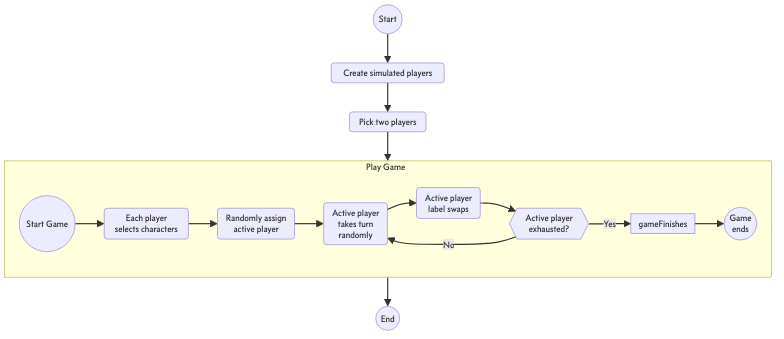
\includegraphics[width=\columnwidth]{60_optimisation_with_aspects/diagrams/naive_model.png}
  \caption{A flowchart diagramming a simple model of RPGLite play, without
  aspects applied.}
  \label{fig:naive_model}
\end{figure}


\inline{Consider changing \cref{fig:naive_model} to only include details about
the model of the game itself, leaving the steps about data analysis to the
later aspect-applied version (which is the real experiment).}
\inline{Move \cref{fig:naive_model} to .svg for fidelity}
The stages of the naive model as laid out map to those encountered by real-world
players. Two randomly-selected players repeatedly select characters to play
(from the pool of 8 characters available in the real-world game), and a player
is chosen to play first at random. That player selects a random valid move to
make.\footnote{Many simulated decisions are random; this is because the model is
designed to be naive, so it avoids informed decisions where possible. Informed
decisions are expected to be woven later as aspects.} The active player alternates, and the process repeats, until
such time as an active player starts their turn with both of their characters
fully depleted of health. The player with remaining characters is the victor,
and another game is started by picking random players and starting a game
between them, until a predetermined number of games has been played.

After a sufficient number of games are played, analysis of the various datasets
collected can begin, although this is discussed in more detail in
\cref{sec:optimisation_with_aspects_experimental_design}.




\section{Experimental Design}\label{sec:optimisation_with_aspects_experimental_introduction}

% Having discussed the naive model above, this section describes how we'll apply
% aspects to set up an experiment, simulating players with variations to
% controlled simulations, and how such an experiment answers our research
% question.

% This likely won't need any subsections: we've already laid out the groundwork
% above as to what's involved technically, so this is statistical, explanation
% of our control, our model under test, and how they'll be compared in a
% rigorous and scientifically appropriate manner.

% However, this \emph{should} lay out the rationale behind simulating learning
% with our aspects; we'll discuss how our datasets are compared here, and how we
% measure similarity, which is done by proportion of classes picked over time.
% There are statistical and methodological requirements at play here --- we
% needed something we could compare in a statistically significant manner ---
% but also, we needed something which the dataset we had could support analysis
% of. We only had a few players with statistically significant numbers of games
% played. Character choice seemed a reasonable way to go, because the metagame
% introduces specific character combinations which are optimal, and we'd expect
% players to learn those over time. Players \emph{might} get stuck in local
% minima, but learning aspects would too, so simulated player data should still
% reflect that. Also, the choice of an ideal team composition is a
% well-understood aspect of metagame design \inline{Is team composition in
% metagame design something there's also literature on, or is this only within
% the gaming industry?}, so we can imagine players optimising team composition
% in RPGLite like they would in other trading card or RPG games.

The naive model above describes a simulation of RPGLite itself; however, the
models exists to support investigation into research questions, and cannot do
this alone. To answer our research questions, the model must be augmented so as
to represent real-world play. This section describes the modifications made to
the naive model (through aspects applied by PyDySoFu) and how data from those
simulations can be analysed to arrive at answers to our research questions. 

The questions these simulations seek to answer are:

\begin{enumerate}
  \item Can we fit model details per-player to get realistic player behaviour?
  \item Can we cluster based on accuracy of different models for each player?
  \item Can we generate predictive data for unknown models from known ones?
\end{enumerate}
% \begin{figure}[H]
% \begin{researchquestion}
%     Can we fit model details per-player to get realistic player behaviour?
% \end{researchquestion}
% \caption*{Research question 1}
% \label{RQ1_experimental_chap}
% \end{figure}
% \begin{figure}[H]
% \begin{researchquestion}
%     Can we cluster based on accuracy of different models for each player?
% \end{researchquestion}
% \caption*{Research question 2}
% \label{RQ1_experimental_chap}
% \end{figure}
% \begin{figure}[H]
% \begin{researchquestion}
%   Can we generate predictive data for unknown models from known ones?
% \end{researchquestion}
% \caption*{Research question 3}
% \label{RQ1_experimental_chap}
% \end{figure}

\inline{These RQs are taken from an early outline of a thesis structure. Maybe they need rewording?}
To investigate these, we produce models of learning which can be applied to the
naive model to augment player behaviour. Simulated players will have their
behaviour augmented in relation to the character pairs they choose to play.
Real-world players could reasonably be expected to choose character pairs which
are stronger together over time. In addition, it is possible to calculate
objectively optimal character pair selections in RPGLite~\cite{kavanagh2021thesis};
therefore, players should be expected to gravitate toward more optimal character
pairs and away from poorer choices as they become more experienced in the game.

A few facets of gameplay are expected to be learned by players over time, and
would theoretically also be suitable objects of simulated players' learning. One
analog to character pair selection could be move selection: players would be
expected to make increasingly optimal moves as they play. However, data can be
muddied by players understanding the optimal use of some characters' moves
better than others, as different characters invite different styles of play.
Small changes to game states (the opposing team's composition, amount of health
remaining, opponent play styles) could influence player behaviour also.
Fundamentally, the state space of moves to be made and scenarios in which to
make those moves is extremely large, making simulation computationally
expensive. By comparison, character selection happens before gameplay starts,
eliminating in-game factors which might influence player decisions.

Modelling the learning of character pair selection allows for modelling of
players learning the metagame, rather than the game itself. Modelling learning
of the metagame allows us to model players learning about the game and other
players' interactions with it, rather than learning the game itself. An example
of the distinction is the difference between learning how optimally make moves
with a Barbarian in a team, and learning the mistakes other players commonly
make when playing a Barbarian to exploit their weakness. As RPGLite is
``solvable'' --- there is a provably correct way to play the game --- players
picking sub-optimal character pairs can be expected to observe that they are
frequently beaten by better ones, increasingly favour pairings they identify as
successful, and so converge on strong character pairs. Convergence en-masse
would indicate a stable metagame. This was observed in practice in real-world
RPGLite play~\cite{kavanagh2021gameplay}. However, while players made fewer
mistakes over time when playing RPGLite, the average cost of a move to their
probability of winning increased after many games (though decreased after a
few).~\cite{kavanagh2021gameplay}. Player behaviour which converges on provably
optimal play is simpler to represent than players' initial improvement followed
by a seeming loss of performance. RPGLite Character selection is therefore a
more convenient metric to model players' interaction with than move selection,
as it presents a smaller state space for simulated players to explore while also
providing a simpler expected end state for those simulated players to converge
to.

Models of learning are therefore applied to players' character selections. Our
primary goal in applying models of learning is to demonstrate whether players
can be accurately modelled by augmenting a naive model to represent them in
particular, thereby answering the first research question. Different real-world
players are expected to exhibit different styles of learning; thus, multiple
models of learning will be applied. Different players might also learn
differently, but in the same style; for example, two players might exhibit
similar biases, but one could be quicker to learn from experience or another
more cautious in the application of new knowledge.

To identify models of learning and parameters for those models which most
realistically represent real-world players, we look to optimise the parameters
for each model, for each player, by running multiple simulations of players
learning in a particular manner (with particular parameters), identifying their
preferred character pairings, and calculating the similarity of the simulated
character pairings to that of a player in the real world. By doing so, we can
anneal to a parameter which represents the optimally realistic model of a player
learning in a given style. If the data produced by this optimally parameterised
model of learning is not similar to empirically sourced data with statistical
significance, we determine that the model of learning applied does not represent
how a player learned in the real world: even the closest dataset the model
produced fit its target dataset poorly. However, if a parameter can be found for
which the model reliably produces character pair preferences which align with
the real-world players' with statistical significance, then the model can be
said to realistically represent that player's learning of the character pair
metagame.

This section will first discuss models of learning generally in
\cref{subsec:models_of_learning_discussed}, and will explain how aspects
implementing these models can be produced in
\cref{sec:optimisation_with_aspects_aspectsdeveloped}. The strategy used to
implement these models of learning is discussed in
\cref{subsec:defining_our_models_of_learning}. The design of experiments
investigating the aforementioned research questions by applying these aspects is
then described in \cref{sec:optimisation_with_aspects_experimental_design}.
\inline{Rearrange either this paragraph of the sections it refers to so they're in order / make sense. At time of writing they refer to 6.3.1, then 6.4, then 6.3.2, then 6.5\ldots{}!}


\subsection{Models of Learning}\label{subsec:models_of_learning_discussed}
Different people learn in different ways. Indeed, no universally-accepted
definition of learning appears to exist. This is presumably because it is
convenient to define what it means to learn differently in the context of
different pieces of work. Cognitive models of learning can be useful when
considering mental processes specifically, for example, whereas functional
models of learning could lend a more empirically applicable perspective. What it
means to learn is clearly outwith the scope of this thesis; however, our
experiments will include models of learning. To justify our model, we consider a
functional approach to learning, as considering learning in this way appears
more closely linked to the empirically focused work of modelling real-world
behaviour than alternatives.

\citeauthor{lachman1997learning} identify\cite{lachman1997learning} that
standard definitions of learning along the lines of, ``Learning refers to a
relatively permanent change in behavior as a result of practice or experience''
have practical shortcomings such as a focus on behavioural change (as learning
may not change behaviour) or conflating learning's process and its product (the
process by which we learn is not obviously identical to its result, of which
behavioural change is an example). They suggest learning might be better defined
as:

\begin{displayquote}
[\ldots{}] the process by which a relatively stable modification in
stimulus-response relations is developed as a consequence of functional
environmental interaction via the senses [\ldots{}] rather than as a consequence
of mere biological growth and development~\cite{lachman1997learning}.
\end{displayquote}

They note that their definition distinguishes learning from phenomena such as
injury, changes to one's maturity, or sensory adaptation, incorporates
stimulus-response relationships the research community consider as learned, and
differentiates learning's process and product. Their model is inherently
functional, making it useful for the purposes of simulation and modelling,
although they offer only a definition of learning and a brief comparison to
the standard textbook definition they introduce. The work presented is not
intended to demonstrate its improved model of learning empirically, only to
discuss its semantic merit. However, the models proposed in this thesis require
only a theoretically informed, sound basis for their model of learning, and a
lack of empirical justification is not a barrier to the relevance of the model
\citeauthor{lachman1997learning} have proposed.

\citeauthor{de2013learning} propose a functional definition of learning which is
primarily concerned with providing a definition of learning which is both
accurate and useful for the purposes of cognitive learning
research~\cite{de2013learning}. Doing so attempts to provide a model around
which some concensus can be reached; learning is a central concept in
psychology, and they see their definition as supportive of cognitive work. They
introduce their definition as follows:

\begin{displayquote}
Our definition consists of three components: (1) changes in the behavior of the
organism, (2) a regularity in the environment of the organism, and (3) a causal
relation between the regularity in the environment and the changes in behavior
of the organism.
\end{displayquote}

This model of learning contains more nuance than the ``textbook definitions'' of
learning they paraphrase as, ``a change in behavior that is due to experience'',
but does not stray far from the core concept: some environmental stimulus
impacts behaviour in a causal fashion. Their introduction of ``regularity'' to
their definition refers to the presence of the stimulus with some form of
repetition, whether this be multiple instances of a stimulus at different times,
or the same stimulus occurring concurrently. \citeauthor{de2013learning} explain
that such a model is straightforward without the sweeping inclusivity of the
simple model mentioned earlier, and is easily verified (although, as in the work
of \citeauthor{lachman1997learning}~\cite{lachman1997learning}, empirical
verification is omitted in favour of semantic analysis).

Aside from other benefits more particular to their research community, these
benefits are especially useful from the perspective of modelling learning in our
case. A simple, functional definition can be captured in a software model, and
introduces few opportunities for misunderstanding or mis-application. It also
introduces helpful concepts --- such as regularity and causality --- which the
other definitions discussed do not. For the purposes of this thesis, we
therefore adopt this definition as a basis for our model of learning.

\subsection{Modelling Learning in RPGLite}\label{subsec:defining_our_models_of_learning}
% Describe our model of learning. Confidence introduces regularity, priors
% introduce causal relationship, behavioural change is in selection of character
% pairs.

We use \citeauthor{de2013learning}'s definition of
learning~\cite{de2013learning} to arrive at a model of learning which is
encodable in aspects that can be applied to our naive model of RPGLite. We are
interested in modelling players learning a preference for character pairs over
time. The model should therefore account for: how player behaviour is influenced
in accordance with their learning, in line with the definition's first
criterion; repetition of experience in successive games influencing the
direction of a player's learning, in accordance with the definition's second
criterion; and do so in a causal manner, in accordance with the definition's
third criterion. We therefore look to model a causal relationship between a
player's observation of successful character pairs and their future choices of
character pairs.

To fulfil these requirements, a model might draw on previously successful
character pairs to determine future ones. There are many ways in which this
could be done. For example, we could model learning as consistently playing the
character pair which most recently was observed to win a game. Any game ending
naturally determines a winning pair, and we can select this pair when playing
future games, until a different pair is observed to win instead. However, this
does not align with our expectations around how players \emph{would} engage with
a game in the real world. Having a strategy one is confident in and being
unlucky with the game's random nature is unlikely to deter a player from what
they believe is ideal. Indeed, we can expect players to understand
that perfect play might not be winning play: in some games, the right moves
might not lead to a successful outcome due to moves randomly missing opponent
characters. Equally, players may take time to become confident in a strategy; we
would expect a player to explore character choices before settling on a
preferred pair early in their experience, and would expect very experienced
players to choose characters based on what they have learned, rather than
continuing to explore options for which they have sufficient information to
reason about. We can infer that:

\begin{itemize}
  \item There are scenarios where players can be expected to observe wins/losses
  without incurring behavioural change.
  \item Players' confidence in what they have learned can affect their
  inclination to draw on what they learn when making decisions.
  \item What players learn in successive games would have a small impact in
  their early experiences, but an increasingly significant impact proportional
  to their experience in the game.
\end{itemize}

% \inline{We've set the stage to explain and justify our own models of learning. Let's go!}
The model of learning used to simulate players' improved play of RPGLite can be
explained following a similar structure: a component pertaining to observations
players make about winning characters; a component pertaining to their inclination
to use that knowledge when choosing characters (rather than exploring their options);
and a component pertaining to the strength of that inclination in proportion to their
experience.

The first --- that players should make observations about winning players --- can
be implemented by modelling the choice as a probability mass function (PMF). The PMF
maps character pairs to their chance of being selected by a player, and initially tracks
all character pairs as having an equal chance of being selected. After every game, the chance
of selecting the winning character pair increases, and the chance of selecting any other pair
decreases. The sum of probabilities of being selected across all character pairs always sums
to 1 (100\%). This can be implemented as a record of the winning character pairs observed by
a player: many ways of producing a PMF from a sequence of wins exist, but for the purposes of
explanation, one such method is to take the proportion of wins for every character pair as 
their probability of being selected. This method produces a valid PMF because the probabilities
must sum to 1 by virtue of the winning pairs being the sole determinant of the probabilities;
every win contributing to the probability of a character pair being chosen means that
100\% of character pairs are considered, and therefore the probabilities inferred from that data
also sum to 1.

A model of learning where prior belief as to optimal character pair is causally related to
those which were previously successful fulfils the first criterion of the model of learning proposed
by \citeauthor{lachman1997learning}~cite{lachman1997learning}; however, players would be expected to
explore a state space in the early stages of their experience. The model proposed by
\citeauthor{lachman1997learning} identifies that the experience of a learning agent draws from
``regularity'' in their environment; we therefore require that an experience affects behaviour
not when it originally surfaces, but after repeated exposure to it. This fulfils the intuitive
understanding of learning discussed earlier --- players' confidence in what they have learned affecting
their inclination to act based on experience --- our second criterion. We therefore require some model of
confidence an agent has in what they have learned.

The third inference --- that confidence should be low initially, and grow proportionally to experience ---
explains the ``shape'' of the confidence model. We require a monotonically increasing function mapping
experience, quantifiable as games played, to confidence, being a percentage chance between 0\% and 100\% that
a player is to determine their character choice based on what was learned, rather than on an exploration of
their space of possible choices.

Such a model of confidence offers a model of learning when combined with a PMF representing historical
observations of a character pair's success.
If the model of confidence indicates that the player is to explore their space of possible choices, they
select character pairs randomly; if they are modelled as confident enough that
their behaviour is instead informed by their experience of their environment,
they select a character pair according to the PMF their historical observations define.
As the PMF affords higher probabilities to repeatedly winning character pairs, player behaviour
is causally affected by the regularity of their experience, implementing a realistic model of learning
in agreement with the functional model proposed by \citeauthor{lachman1997learning}~\cite{lachman1997learning}.

Our model of learning is therefore complete, but a model of confidence remains to be defined.

\subsection{Modelling Player Confidence in RPGLite}\label{subsec:confidence_model}

To model learning, we must find some function mapping experience (quantified by
a count of games played) to some probability between 0 and 1, and fitting the
criteria described in \cref{subsec:defining_our_models_of_learning}.

A sigmoid curve fulfils both the second and third inferences in
\cref{subsec:defining_our_models_of_learning}. It also notionally conforms to
expectations around ``confidence'' as an anthropomorphic trait: much like a
sigmoid, confidence starts low, and remains so until it achieves some inflection
point, after which it grows rapidly until tapering asymptotically toward some
maximum. However, not all real-world players might express the same traits in
their growth of confidence; the shape of their sigmoidal confidence may differ.
In order to account for this while guaranteeing a monotonically increasing
mapping of the number of games played to a player's confidence, we select a
sigmoid which can be parameterised to alter their shape.

A sigmoid curve is suitable for this model of learning where other curves would
not suffice, because we require a period where players lack confidence and
explore their options. Sigmoid curves such as the
logistic~\cite{verhulst1845loi} or Gompertz~\cite{gompertz1815curve} are widely
used when modelling systems~\cite{werker1997modelling}, but while they fulfil
the role of a monotonically increasing curve with asymptotically low and high
initial and final states, the shape of such curves is not trivially modified to
fit different players' learning styles.

More flexible asymptotic curves were developed by
\citeauthor{richards1959flexiblegrowth}~\cite{richards1959flexiblegrowth} drawing on growth curves developed by
\citeauthor{von1938quantitative}~\cite{von1938quantitative}, which afford a natural pattern of growth;
\citeauthor{richards1959flexiblegrowth} amends this curve to offer a parameterised growth rate. This curve
can be made equivalent to other curves, including the logistic and Gompertz~\cite{france1984mathematical}.
This curve allows for a parameterised rate of growth, but lacks parameters controlling the points at which
growth occurs most rapidly. The relative rate of confidence gain is a separate concern to the point at which
such growth occurs: a player might cautiously grow in their confidence until they are already very experienced, or
might bullishly grow in confidence yet plateau early, taking longer to reach complete confidence in themselves
than they did to garner an initial increase, regardless of their relative growth in confidence.

The flexibility of a parameterised relative growth rate appeals to the notion that different players would
gain confidence at different rates, but the point at which confidence accelerate most must also be controlled.
We therefore employ the Birch curve, proposed by \citeauthor{birch1999new}~\cite{birch1999new} for
its increased flexibility as compared to the Richards curve combined with its additional parameter used to control
the curve's shape.
\footnote{\citeauthor{birch1999new} refers to shape to mean the point of inflection of a curve. The point
of inflection of an exponential rise to a limit is at its initial point; the point of inflection of the
logistic curve is in the exact midpoint of the curve's growth.}
Different players might exhibit different rates of growth in their confidence, and might grow maximally in their
confidence at different points in their experience; the birch curve satisfies these properties as a model of
confidence.
\inline{Investigate: did we ever model confidence with anything other than c==1, i.e. a standard logistic curve?}


\section{Aspects Applied}\label{sec:optimisation_with_aspects_aspectsdeveloped}

% Players can be expected to select stronger characters as they understand
% gameplay more. Aspects were therefore developed to track player experience with
% characters. As players became more familiar with the characters they play, we
% can hypothesise that they will better understand how to play with those
% characters, and more often select characters they have success with. 



% \inline{Write about \emph{both} aspects so as to answer the hypothesis : Can
% aspects be used to generate models of alternative behaviours?}

% The aim of this experiment is to investigate whether a model with
% aspect-oriented behavioural variation can be realistic; the experiment therefore
% requires the development of aspects representing plausibly realistic behavioural
% variation. Traces from simulations affected by these aspects should produce
% synthetic data which can be compared to real-world data and to naive data,
% enabling the measurement of the datasets' similarity, as discussed
% in~\cref{sec:optimisation_with_aspects_aspectsdeveloped}. 

% To demonstrate that simulated players are plausibly realistic, and
% that a simulation's realism can be improved by the addition of behavioural
% variance as a cross-cutting concern, naive player behaviour is augmented by
% applying aspects which represent learning. Two methods of learning RPGLite's
% metagame were produced; this section will detail both.

% In each model of learning, players are assumed to have a draw towards choosing
% to play some characters, and less of a draw to others. This draw is informed by
% whether players have reason to believe they'll be successful after choosing a
% given character; players' future decisions are informed by the outcomes of their
% previous ones. The models of leaning presented in this section are
% differentiated by the manner in which future decisions are informed.

Having a naive model of player interaction in RPGLite allows for the generation
of a control dataset, which can be compared to aspect-applied datasets to
examine whether the aspect-applied models are provably ``closer'' to
empirically-sourced data than the naive dataset\footnote{``Closer'' here refers
to a similarity measurement which we will define later in this chapter.}. To
generate the experimental dataset, the naive model producing our control is
augmented through the application of aspects. These aspects fulfil different
functions, and can broadly by grouped into three categories:

\begin{enumerate}
  \item Aspects implementing behavioural models, changing the behaviour of
  simulated players;
  \item Aspects instrumenting the naive model to perform observations necessary
  for the implementation of behavioural models (such as models of learning) on
  the naive model;
  \item Aspects altering the behaviour of modelled players to simplify
  experimental observation, and to handle exceptions introduced by changes
  within the aspect-applied model.
\end{enumerate}

The first set of aspects implement the behavioural change we anticipate will
produce datasets closer in similarity to empirically sourced data than that
sourced by the naive model. The second set lays the foundation for applying
these changes. The third applies behavioural changes which experimental
observations require. Necessary changes unrelated to our models of learning will
first be explained in \cref{subsec:aspects_improving_model}, followed by an
introduction of foundational observations for our models of learning in
\cref{subsec:aspects_modelling_learning}. Finally, the models of learning built
on those foundations are introduced in
\cref{subsec:aspects_instrumenting_model}.
\inline{The ordering of this explanation of different uses of aspects is confusing; once the aspects are explained individually, reorder the sections, rework the introduction to the structure of this section, and ensure the outline of the section reflects the changes made.}

\begin{figure}
  \centering
  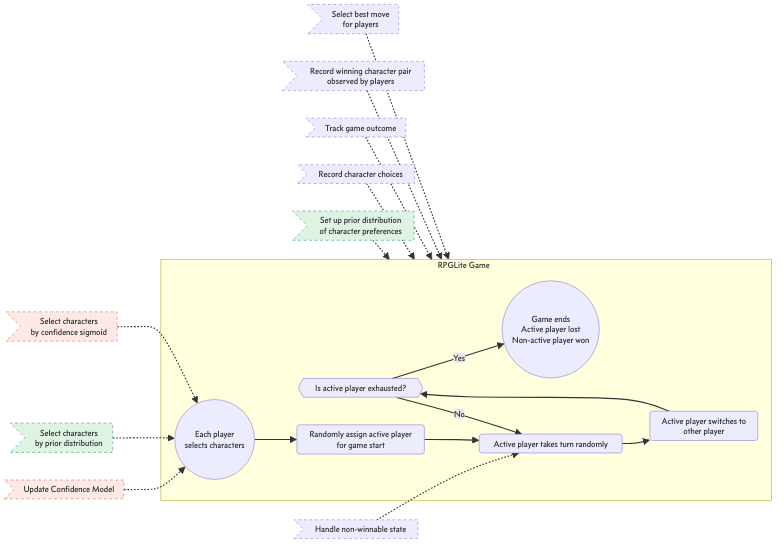
\includegraphics[width=\columnwidth]{60_optimisation_with_aspects/diagrams/aspect_applied_model.png}
  \caption{A flowchart describing a simulated game of RPGLite, and all aspects woven into the game to implement the various models of learning. Some aspects should not be woven together in the same experimental run, as they implement different models of learning.}
  \label{fig:all_aspects_applied}
\end{figure}

A diagram of a game of RPGLite with all possible aspects
applied\footnote{Including aspects which should not be woven in the same
experimental run: some aspects implement different models of learning and are
therefore conceptually incompatible.} is
presented in \cref{fig:all_aspects_applied}, by way of high-level overview of
the aspects this section introduces.

\subsection{Aspects for model improvement}\label{subsec:aspects_improving_model}

\subsubsection{Ensuring the Best Move is Played}\label{subsubsec:ensure_best_move}

% We make sure players always make the best moves, because it reduces the space of
% situations where randomness can skew our results. An analysis of how well this
% reflects real-world player interactions can be found in \inline{Cite William's
% thesis for realism of players making perfect moves.}

As discussed in \cref{sec:optimisation_with_aspects_experimental_introduction},
the goal within this experiment is to build a model of players' learning of
character selection rather than move selection. However, randomly selected moves
are liable to place players in unrealistically weak positions, as players are
unlikely to make obviously poor moves such as skipping a turn with no clear
reason. It would be unexpected to see true randomness in players' moves. This is
a concern for the modelling of players' character selection, because the model
of learning defined requires a causal relationship between what is observed (in
this case characters which most reliably win games) and behavioural change
(players choosing character pairs proportionally to their estimated chance of
winning a game); if selecting random moves cause simulated players to lose games
when they would have realistically won them, this would affect character
selection by definition.

Character selection and move selection are therefore somewhat linked. However,
move selection is most frequently optimal: in the majority of cases real-world
players chose the best move available to them, as analysed by \citeauthor{kavanagh2021gameplay}~\cite{kavanagh2021gameplay}~:

\begin{displayquote}
  [\ldots{}] the majority of actions taken were optimal, with a cost of 0.0. In
  total 73\% of the player’s season 1 actions and 77.8\% of their season 2
  actions were optimal.\footnote{Different seasons of RPGLite are discussed in
  more depth in \inline{Make a reference to the chapter(s) where I explain
  different seasons of RPGLite.}}
\end{displayquote}

Therefore, a naive model of move selection which represents real-world move
choices in \(\frac{3}{4}\) of cases is to select the best move at every
opportunity. We therefore apply an aspect to the function responsible for move
selection which performs a lookup on the dataset of action costs defined by
\citeauthor{kavanagh2021gameplay}~\cite{kavanagh2021gameplay}, and select the
known-optimal move in every case.

One additional factor in move selection is handled by this aspect. As simulated
players' behaviours are augmented to select universally optimal moves, an
anomaly in the dataset was identified. In some games, optimal play would result
in infinite loops: players would arrive in a state where they would skip turns
mutually and indefinitely. This is because it is possible that, in RPGLite, to
make any move is disadvantageous. \footnote{This is because barbarians deal more
damage once they lose a sufficient number of hit points. As a result, to deal
damage to a barbarian can result in their having an opportunity to win in one
move rather than two in certain health states.} Both players can concurrently
exist in this state. Therefore, both players' optimal move is to skip their
turn. \citeauthor{kavanagh2021gameplay} note that such states were reached in 64
cases in real-world play, but real-world players never skipped their turn;
therefore, this scenario is also an example where suboptimal play can be
re-introduced. This aspect therefore returns random moves if the previous two
moves in a game were to skip. Such a state indicates that the game reached a
stable point where neither player would optimally deal damage to the other.
Random moves destabilise this state and return to ordinary play.

A model of move selection more closely aligned with expectations of player
behaviour is beyond the scope of this thesis: a demonstration that models of
both move selection and character selection can be optimised concurrently to
arrive at a realistic model of empirical play with multiple aspectually applied
models of behavioural variance invites itself as future work.
\inline{Do I need code snippets for notes on aspects?}


\subsubsection{Handle Game States with no Viable Moves}

% Using lookup tables provided by William's thesis (cite here!) means
% crossreferencing the game states in our simulation against game states in
% William's models. Turned out there were states they didn't track because it
% was not possible to make any move at all that could win, so the game's a
% foregone conclusion in those states. Because the aspect in
% \cref{subsubsec:ensure_best_move} aspect reads states from lookup tables which
% might not contain those states, our model can throw exceptions when performing
% lookups! Handle those scenarios and treat as an unwinnable game for the
% appropriate player.

A consequence of playing games using only optimal moves was that unexpected
states could occur. One might assume that, choosing moves optimally from a
dataset of available moves in every game state it would be infeasible to arrive
at states not present in this dataset. However: the dataset was produced through
model checking, with the aim of identifying the cost of an action regards its
impact on a player's chance of winning. If a loss is guaranteed, all moves have
a 0\% chance of winning; the model checker producing the dataset of available
moves therefore identifies that the game is a foregone conclusion, and contains
no valid moves. 

In such a situation, identifying the winning player is as simple as identifying
the player who made the previous move. We therefore apply an aspect which handles
exceptions raised by move selection (as lookups will fail due to the game's current
move state not existing in the dataset of action costs) and, after identifying that
the exception indicates that the state does not exist (in this case, a 
\lstinline{KeyError}), the aspect handles the exception by assigning the losing player's
characters 0 health and swapping active players so that the simulated game proceeds with
the losing player taking the following turn. As this turn starts with the active player
having 0 health, the game ends as expected.


% TODO: Section / subsection for observational aspects
\subsection{Aspects for Instrumentation}\label{subsec:aspects_instrumenting_model}

As explained in \cref{sec:optimisation_with_aspects_aspectsdeveloped}, the experiment
being discussed requires observational apparatus to be implemented in order to
collect data about the experiment for later analysis. Ordinary experimental setups
might require this apparatus to be tangled through the experimental codebase; however,
aspect orientation provides a technique for augmenting the simulation to make observations
before, during, or after any step of within the model. This demonstrates observational
scaffolding as a cross-cutting concern as suggested by~\citeauthor{gulyas1999use}~\cite{gulyas1999use}.
Aspects realising this concept and supplying observations and additional models in support of our
model of learning are discussed here.


\subsubsection{Update Model of Confidence}

The models of learning described in \cref{subsec:aspects_modelling_learning} have players
make observations as to the character pairs which most frequently win games, and
have those players alter their behaviour in response to these observations. However,
as discussed in \cref{subsec:confidence_model}, a model of confidence is required to complete
our model of learning. This model of confidence is a sigmoid curve, and the Birch curve was selected
for our model of confidence. The role of this aspect is to update the birch curve when a game ends.

An aspect updating our model of confidence is applied to act after a game ends (an ``encore'' in
PyDySoFu's parlance), and updates a value in the model's environment for confidence models. Confidence
is represented as a mapping of player objects to floating point values between 0 and 1. The aspect supports
modelling confidence in many ways, identified by a \lstinline{sigmoid_type} parameter within the model's environment.
% However, the model was executed using a \lstinline{birch_c} logistic curve, which implemented the 
\inline{OH NO. I just realised our models don't use birch at all, they use a logistic curve.
They also use a relative growth rate on the logicstic curve that I'm unsure of — not sure why I implemented
it the way I did.
Getting increasingly close to just re-running my models. I could run them again using birch, and maybe anneal to
a value for the curve shape for different players too...?! THIS NEEDS TO BE FIXED ASAP.}

\begin{enumerate}
  \item A logistic curve
\end{enumerate}



\subsubsection{Record Prior Distribution of Character Preferences}
% \inline{Looks like aspect recording prior distribution might be applied to data
% generation; figure out how to fit it into \cref{fig:all_aspects_applied}.}

%% IMPORTANT NOTE TO SELF
%%
%% The reason we have a prior is because it's being calculated on TRAINING DATA.
%% The training fold contains a bunch of data which we use as our prior when picking future
%% character pairs under some models.
%% I need to look more into this but I'm certain it's what's happening.
%% I _definitely_ need to think more about why I did it this way, and find some notes / messages
%% from around te time to load back up what my train of thought was vis-a-vis using the training fold
%% in this way. I guess the idea was to use the training fold as a starting point for the model, and then show that
%% we can use it to "fill in" gaps in the dataset by producing similar information to what's in the 
%% testing fold, but it feels unusual; need to properly understand this.
%%
%% END IMPORTANT NOTE TO SELF

\inline{Keeping this in because I might need to explain the aspect, but it's only
used in the implementation of choosing based on prior distribution, which I don't
believe is ever applied. So! Decide whether to get rid of the writeup of that model.
If I \emph{am}, then get rid of this too. If not, add it to the learning models writeup
below and explain it here.}

\subsubsection{Record Character Pair Choices}
It is important to keep track of the characters chosen by simulated players, as this data is
required to analyse the outcome of the experiment~\inline{Do we describe an experiment singular or experiments plural in
\cref{chap:exp1_simulation_optimisation}?} outlined in this chapter. However, the naive model makes
no special accommodation for the collection of character choices made by players. Character choices could
be calculated by iterating through the list of completed games after a simulation is complete, filtering
for games relating to a specific player. However, the collection of character selection data can be simplified
by tracking what was played at the end of a game.
This is achieved with with an
aspect which observes the character pairs played in a completed game, and appends each players' chosen pairs to their own list.
This aspect is applied after
its join point executes (an ``encore'' in PyDySoFu parlance\inline{reference pdsf's explanatory chapter
/ re-engineering chapter here? unsure which is most appropriate / introduces the concepts first.}).

There are many ways to collect this data, aspectually or otherwise; however, the simplicity of collecting information mid-process
without requiring modification of a base model demonstrates the flexibility of an aspectual augmentation of models and simulations
as an approach. Collection of chosen character pairs mid-simulation is an opportune example of this convenience.

\subsubsection{Track Detailed Outcomes of Games}\label{subsubsec:detailed_game_outcome_tracking_aspect}
Similarly to the recording of character pair choices, the outcomes of games must be tracked. This information
is important as an input of our model of learning, as successes and failures observed by players for each character pair
can inform their models of learning. Some models of learning implemented, such as one including a hyperbolic decay bias
(to be explained later, in \cref{subsubsec:learning_with_hyperbolic_decay}), require not only knowledge of the proportion of wins
each character pair has achieved, but also the history of wins and losses: players might be biased toward recent win/loss observations,
discounting older experiences in favour of the new. Detailed historical win/loss information must therefore be recorded.

As with character pair choices, the naive model was not engineered with the intention of providing this information specifically.
However, the model is easily instrumented to collect such information at many suitable points. As with recording
a player's chosen character pairs, an ``encore'' aspect was implemented which records wins and losses observed for character pairs
on game end. Specifically, the aspect models players observing character pairs which won at the end of a game, lost at the end of
a game, and also pairs which were uninvolved in the game. This requires a list of outcomes (wins, losses, and neither) for every player, for every character pair.
The lists of observed outcomes for a given character pair record 
\lstinline{True} for a winning pair, \lstinline{False} for a losing pair, and \lstinline{None} for a character which was not
involved in the game's outcome. Each player observes the relevant state for every character at the end of any game they play. 
Provisions were made in the implementation of this aspect for a player only paying attention to
their own outcomes (i.e. only recording whether their own pair won or lost, without consideration for their opponent's outcome),
though in practice all simulations were performed with players observing both their own outcomes and those of their opponents.

\subsubsection{Record Winning Pair observed by Players on Game End}\label{subsubsec:aspect_to_observe_winning_pair}
Unlike the detailed game outcome data recorded by the aspect described in \cref{subsubsec:detailed_game_outcome_tracking_aspect} and used
in advanced learning models such as that of hyperbolic decay (to be explained later, in \cref{subsubsec:learning_with_hyperbolic_decay}),
other learning models required only simple outcome data. The simpler model of learning making use of
a distribution of winning teams to be explained in \cref{subsubsec:learning_by_picking_from_distribution_of_wins_with_confidence}
is more easily implemented against a simple list of winning teams. Rather than coalescing the more complex dataset collected as described in
\cref{subsubsec:detailed_game_outcome_tracking_aspect} to achieve the desired format, another aspect can be applied
to collect the data in a simpler format directly.

An aspect was implemented which also models players observing winning character pairs on game end, but collects the data in a
simple list of character pairs observed to win games, rather than a mapping of character pairs to game end states as described in
\cref{subsubsec:detailed_game_outcome_tracking_aspect}. Character pairs which lose games or are not involved are not recorded for the purpose
of the alternative model of learning.

% TODO: Section / subsection for models of learning
\subsection{Aspects Implementing Models of Learning}\label{subsec:aspects_modelling_learning}

% * The aspects already described explain how we set up the model for applying our learning implementations,
%   both instrumenting it for observation and tweaking fundamental behaviours.
% * Now we need to implement models of learning! We'll present two.
% * First, a simple model of learning as described in \cref{subsec:models_of_learning_discussed}
%   which uses a confidence sigmoid to discern between selecting character pairs based on what was 
%   previously observed to win games, and random selections representing exploration of a player's options.
% * Second, a more complex model of learning which applies the same concepts, but introduces a hyperbolic decay
%   on the simulated player's learning, introducing a biased model of learning.

The aspects described above implement setup for the models of learning applied in this thesis,
both instrumenting the underlying RPGLite model for observation and tweaking behaviours of the naive model.
Two aspects remain unexplained, implementing the learning models themselves.

The first model of learning left to be described is implemented as described in
\cref{subsec:models_of_learning_discussed}, drawing from a record of character pairs observed to win
in earlier games to select characters in future games, in accordance with a model of confidence which activates
either this behaviour or a randomly selected pair. A detailed description follows in
\cref{subsubsec:learning_by_picking_from_distribution_of_wins_with_confidence}.

The second model of learning left to be described
implements a similar logic, but introduces a weighting on the history of winning pairs a player
observes, introducing a hyperbolic discounting bias to historical observations. 
In this model, players increasingly discount old observations in favour of recent ones. A model of learning with
a hyperbolic discounting bias is described in
\cref{sec:optimisation_with_aspects_experimental_design}.

\inline{Why didn't we make a bayesian model of learning? Should we have? Would this be difficult at all?}

% \subsubsection{Character Selection from prior distribution}
% ==== NOTE: the above subsubsection references an aspect where characters are picked directly from
%            the prior distribution from a training set, and doesn't contain a model of learning at all.

\subsubsection{Character Selection using confidence sigmoid}\label{subsubsec:learning_by_picking_from_distribution_of_wins_with_confidence}

The first model of learning applied through aspect orientation draws on character pairs a 
simulated player observed to have won games (as recorded by the relevant instrumenting aspect,
discussed in \cref{subsubsec:aspect_to_observe_winning_pair}). The record of previously winning character
pairs defines a probability mass function by selecting a character with equal probability to
their rate of appearance in the history of winning characters.

Selecting a character based on this
distribution is gated by a confidence model as described in \cref{subsec:confidence_model}. If a
simulated player's confidence model indicates insufficient experience to found decisions on, players
will instead select characters randomly, effectively exploring their space of possible choices.
By doing so, players have the time and opportunity to observe many matchups between different character pairs.
Time to observe matchups is important because some character pairs may only present a strong choice
if played against specific alternatives.
We can imagine a character pair which is extremely effective against 50\% of pairs, but extremely likely
to lose games played against the remaining 50\% of possible opponents. Without exploring possible matchups,
a player may lack observations which would inform them about whether a character pair is effective in general, or
in a narrow set of circumstances. A confidence model encouraging early exploration promotes the experience
of a wide variety of matchups, avoiding this issue.

Another concern early exploration mitigates is that simulated players need opportunities to build
well-rounded priors: if a character pair is never selected by any player, experienced players basing their
character pair choices on those which previously win games cannot include pairs which were never selected,
because they will never have had the opportunity to win games at all.

This aspect was implemented as an ``around'' aspect in PyDySoFu's parlance, allowing it to
apply additional logic before and after its join point. It could equally appropriately have been
implemented as an ``encore'', applying logic only after its join point had executed; the aspect
discards the random selection made by the base model unless the simulated player lacks confidence.
Either implementation can return a different character pair choice to the join point's caller, allowing
the chosen character pair to effectively be overridden, and so allowing the aspect-applied RPGLite model to
proceed executing as it would otherwise; the only difference being the pair of characters ``chosen'' by the
simulated player whose behaviour was augmented.


\subsubsection{Character Selection exhibiting hyperbolic decay}\label{subsubsec:learning_with_hyperbolic_decay}

Character selection with hyperbolic decay works similarly to the simple model of learning
as described in \cref{subsubsec:learning_by_picking_from_distribution_of_wins_with_confidence}.
Character pairs are selected randomly if a player lacks confidence or, if the confidence model applied
to the player indicates that character pairs are to be chosen according to their historical observations of
winning pairs, their record of winning pairs in previous games informs their choices instead. However,
this model also applies a hyperbolic discounting bias which weights the player's historical observations
when making choices.
\inline{Maybe we should have also produced models of other discounting mechanisms, like exponential discounting
(which I \emph{believe} is actually the logically sound way to discount). Would be interesting to see
whether some players are well-modelled by other discounting mechanisms. Investigate this!}

Hyperbolic discounting is a bias studied in behavioural economics.
\inline{Find citations explaining hyperbolic discounting}

A hyperbolically discounted score for an event after a delay \(D\) with discounting factor \(k\) is
calculated by:

\begin{figure}
\[score(D) = \frac{1}{1 + kD}\]
\caption{Hyperbolic discounting score calculation}
\end{figure}

This score can be applied to a history of games played with different character pairs to weight that history;
this weighting can then be used to create a new PMF to draw character pair choices from, by allocating each pair
a probability of being chosen according to its share of the weighted history of winning pairs.
Where the previous method for selecting character pairs selected each pair with the frequency they appear
in the record of winning pairs, this method weights the record of winning pairs; the sum weighted history of
a character pair's wins as a proportion of the total weighted history for all pairs
becomes the PMF for character pair selection.
\inline{Maybe there's need here for a diagram or some extra equations to make this clearer\ldots{}?}

With this scoring mechanism, our model of learning incorporates a behavioural bias which some real-world players
may exhibit. Player character choices can now be modelled through different behavioural variations applied to the 
naive model. The resulting behaviours from each model of learning can be compared to that exhibited by the naive model
to discern which produces simulated RPGLite play more similar to a given real-world player's;
methods for doing so are explored in the remainder of this chapter. 

\section{Experimental Design using Aspectual Learning Models}
\label{sec:optimisation_with_aspects_experimental_design}

% Specifics of how we intend to analyse our data, leading on from the brief
% discussion in \cref{sec:optimisation_with_aspects_experimental_introduction}.
% \inline{Discuss specifics of how we intend to analyse data, rather than high-level experimental overview presented in earlier chapters}

The models of learning described in \cref{subsec:aspects_modelling_learning} can
be applied to augment the naive model described in
\cref{sec:optimisation_with_aspects_naivemodel} and introduce change in player
behaviour over time. The remaining challenge is to demonstrate that augmenting
the naive model can make it more realistic in practice. To that end, the
remainder of this chapter details an experiment which compares synthetic
datasets produced by the model to empirically sourced data, and shows that this
synthetic data is quantifiably more similar to its empirical counterpart than
that produced by a naive model with no aspects applied.

This section presents the strategy for generating synthetic datasets with
aspects applied, comparing simulated and real-world play, and describes the
strategy used to analyse results.

\subsection{Quantifying Similarity of Character Pair Selection}

% The research questions which these experiments aim to answer require a method
% for comparing the similarity of character pair selection in a given instance
% of simulated play. Quantifying how similar a simulated player's character pair
% selections are to their real-world counterpart allows such a comparison. The
% goal of this comparison is to determine whether synthetic datasets of
% character pair choice data align closely with empirically sourced datasets
% insofar as this comparison investigates whether real-world players are more
% accurately modelled in one simulation than another; 

% What do I want to say here?
%
% * We need to compare distributions of choices rather than choice history
%   because we'd expect natural variations, and what matters is whether players
%   ended up choosing similarly as they learned
% * A distribution gives us a ranking of choices; we can see preferences. We're
%   therefore interested in whether players consistently ranked certain
%   character pairs over others.
% * There's lots of RNG in RPGLite, so the degree to which those character pairs
%   are picked is a tricky thing to get right. It's also not necessarily a good
%   measure of similarity: whether players learn can be measured in a bunch of
%   ways, and similar _proportions_ is a harder bar to reach than similar
%   rankings.
% * It matters that we're not interested in similar proportions because it
%   changes the correlation metrics we use to measure. Our aim is to show that
%   the aspect-applied model is "more realistic". We can decide what that means.
%   If players get the character pair preferences right, surely that's enough
%   for us.
% * We can't predict much about our data because different players might have
%   different properties to their character pair choices, _but_ we can make zero
%   assumptions about the data by using an appropriate technique to calculate
%   similarity. Non-parametric rank coefficients tell us how closely associated
%   two rankings are. Two major choices are Spearman and Kendall; we opt for
%   Kendall because Spearman's is sensitive to discrepancies between rankings,
%   rather than simply whether the rankings are concordant. Character pairs
%   which aren't chosen often are likely to have large discrepancies in rank but
%   small discrepancies in their rate of choice, and we shouldn't penalise a
%   dataset for having similar rates of choice but dissimilar rankings in the
%   tail of the distribution of character pair choice.
% * We can get the pvalue of two datasets being associated directly from scipy's
%   implementation of Kendall's Tau; so, we can use the pvalue of the datasets
%   being associated as our similarity metric.

% * We need to compare distributions of choices rather than choice history
%   because we'd expect natural variations, and what matters is whether players
%   ended up choosing similarly as they learned

\inline{This subsection most likely needs to be condensed.}
The experiments presented in this chapter make comparisons of many synthetic
datasets to a single empirically sourced dataset. The latter contains all games
completed by a player whose learning of RPGLite we aim to simulate, and is drawn
from the published RPGLite dataset~\cite{rpglite_dataset}. The comparisons are
required to determine which of the synthetic datasets most closely matches the
empirical dataset. We are specifically interested in determining whether players
played with preference toward similar character pairs. The distribution of their
choices describes a bias toward some pairs, and away from others. The
distribution of the naive model, being randomly chosen, should exhibit no bias;
a simple null hypothesis is therefore that a simulated dataset is as similar to
real-world play as a randomly generated one; there exists no bias comparable to
that exhibited by the empirical dataset in this case. Our hypothesis in
answering the first research question posed is that, with models of learning
applied through aspect orientation, the naive model can exhibit biases toward
character pairs similar to that of a real-world dataset. The simulated play
would therefore exhibit a more ``realistic'' behaviour in character selection
than the naive model as a result of the aspects applied.

% * There's lots of RNG in RPGLite, so the degree to which those character pairs
%   are picked is a tricky thing to get right. It's also not necessarily a good
%   measure of similarity: whether players learn can be measured in a bunch of
%   ways, and similar _proportions_ is a harder bar
% * A distribution gives us a ranking of choices; we can see preferences. We're
%   therefore interested in whether players consistently ranked certain
%   character pairs over others.

We expect discrepancies in the specific character pairs selected in games (such
as the order of character selection) because of the random nature of character
selection. However, it is feasible to assess the similarity between the
distribution of character pairs chosen by simulated and real-world players. The
distribution of a player's chosen character pairs describes the preferences of
that player, as it allows their selections to be ranked. We can examine the
similarities between a player's character pair preferences and the preferences
of simulated players by ranking and correlating their preferences to arrive at a
measurement of similarity between the datasets; this is achieved through
rank correlation.

Many rank correlation measurements exist. For the purpose of comparing lists of
character pairs, we require a non-parametric measurement. Some methods for
calculating correlation assume a distribution of data, or require data to be
distributed in a consistent manner; as nothing is known about the distribution
of character choice preferences (and this distribution could vary between
players), a measurement which is independent of the underlying distribution is
required. Two common options are Spearman's \rho and Kendall's \tau.
\inline{Find citations for each correlation coefficient, and also for justifying choosing between these two specifically (if required).}
These measurements assess correlation in different ways, which can affect
measurements of character pair preference. Spearman's \rho accounts for the
magnitude of difference between ranks, and is calculated as $\rho = 1 - \frac{6
\sum (d^{2}_{i}}{n(n^{2}-1)}$, where $d^{2}_{i}$ is the difference in the rank
of the $i^{th}$ observation in each dataset and $n$ is the total number of
datapoints in a dataset. Kendall's \tau{} accounts only for their ordering. It
can be calculated as $\tau = \frac{C - D}{C + D}$, where $C$ is the count of
concordant pairs, and $D$ the count of discordant pairs.

To choose an appropriate measure, we relate them to potential patterns in our
datasets. As we expect many character pairs to be infrequently picked (if at
all) once players develop preferences, a slight increase in selecting uncommon
character pairs within a simulation could incur a significant increase in rank.
This would have a more significant impact on \rho{} than on \tau{}, as the
larger difference in rank is squared in the calculation. The simulated dataset
might also produce a distribution where rankings between empirically sourced and
synthetic datasets had small differences, but were similarly positioned
throughout the dataset. This would have an outsized impact on \tau{}, as
relative positioning affects concordance, but the square of a small difference
in rank remains relatively small, meaning that \rho{} would be less affected by
this pattern. A choice of correlation metric is thus a choice of what
correlation means: should correlation more closely reflect preference of
character pairs relative to each other, or ``forgive'' small relative preference
deviations but impose a greater cost on the scale of disagreement on a given
rank?

% We choose to prioritise the preservation of rank order over the minimisation
% of rank difference. This is because character pairs which are infrequently
% chosen may have significant differences in rank as they are likely to have
% similar, extremely low rates of selection. Differences in the rank of
% unfavoured character pairs might be In addition, preserving the ordering of
% frequently chosen character pairs' preferences would indicate similar choices
% for the majority of games played when players exhibit strong preference for a
% small subset of available pairs, and would also punish 

We choose to prioritise the preservation of rank order~(\tau{}) over the
minimisation of rank difference~(\rho{}). Unfavoured character pairs' ranks
might be affected greatly by a small difference in the number of games played,
because unfavoured character pairs play few games by definition. A small
difference in selection count is therefore more likely affect rank; however, the
character pairs would still be unfavoured relative to a players' preferred
pairs, which are expected to have a disproportionately high number of games,
also by definition. Minimising rank difference is therefore sensitive to
RPGLite's random nature. Preserving the ordering of character pair selection is
also important when considering favoured pairs, as differences might indicate a
difference in patterns of play; however, small differences in the ranks of
favoured pairs with \rho{} would have a less signifiant impact than when
measuring rank ordering with \tau{}: \rho{} accounts for the square of the
difference in rank, which remains small for small differences.

For these reasons, we quantify similar character pair preferences by
representing preference as an ordered list of string-represented character
pairs, and measuring their correlation using \tau{}.
\inline{I'm not sure I've defined how I represent (or calculate) the ordered list of preferences yet. If not, that should live somewhere, I suppose.}


\inline{230829: I'm here at time of writing.}

\subsection{Producing Datasets}

% A brief explanation of `generate_synthetic_data`, to separate it from the
% annealing below.
% It's responsible for:
% - Setting up special vals consumed by aspects in the games' environment dict
% - weaving aspects (and un-weaving them)
% - matching players together and kicking off games
% - Recycling players when they get ``bored''

Our goal is to produce datasets of simulated player behaviour with aspects
applied. This is achieved through the naive model's \lstinline{play_game}
function. Related work also exists to manage the environment games are played
within, manage the simulated playerbase, and weave \& remove any aspects. The
experimental codebase contains a function, \lstinline{generate_synthetic_data},
which is responsible for this related work. 

% Special vals in environment for different aspects we might apply
% Weaving aspects, unweaving at the end
% creating and matching synthetic players
% Model of boredom (which can be switched off, importantly)


\subsection{Annealing toward Player-Specific Learning Parameters}

\inline{Discussion required here around the mitigation of randomness --- it's
required because of RPGLite's inherent RNG --- and also explaining how we make
use of a grid search in combination with k-fold validation to anneal toward
well-fitted parameters of our models of learning for each individual player.}

\inline{TODO make a diagram of this.}

% To mention here:
% \begin{itemize}
%   \item Data generation specifically: \begin{itemize}
%     \item Boredom. We rotate players to make sure we've got a constant stream of
%     new players being introduced into the game, and to maximise the number of
%     times a simulated player is able to explore the state space.
%     \item Data generation
%     \item normalisation.
%     \item Calculation of preference distribution lists
%   \end{itemize}
%   \item Actual annealing: \begin{itemize}
%   \item Identify the different parameters to fit, and briefly explain them and
%   their significance to the model.
%   \item Testing combinations of different parameters. Compare grid search on RGR
%   to current combine-lots-of-parameters technique.
%   \end{itemize}
% \end{itemize}



\section{Experimental Results}
\label{sec:optimisation_with_aspects_experimental_results}

Presentation of the results owing from the experiment as described in
\cref{sec:optimisation_with_aspects_experimental_design}, and evaluation of the
research question with respect to these findings.

Again, no subsec likely required here.

\section{Discussion}
\label{sec:optimisation_with_aspects_discussion}

A closing discussion on what we found, and how the research question was
answered.